\item A plank of mass $m_1$ with a bar of mass $m_2$ placed on it lies on a smooth horizontal plane. A horizontal force growing with time $t$ as $F = at$ ($a$ is constant) is applied to the bar. Find how the accelerations of the plank $w_1$ and of the bar $w_2$ depend on $t$, if the coefficient of friction between the plank and the bar is equal to $k$. Draw the approximate plots of these dependences.
    \begin{center}
        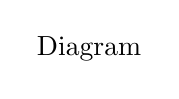
\begin{tikzpicture}
            \node at (0, 0) {Diagram};
        \end{tikzpicture}
    \end{center}
    \begin{enumerate}
        \item Find how the acceleration $w_1$ depends on $t$.
        \item Find how the acceleration $w_2$ depends on $t$.
        \item Draw the approximate plots of these dependences.
    \end{enumerate}
\begin{solution}
    \begin{center}
        \begin{tikzpicture}
            \pic at (0, 0) {frame=3cm};
        \end{tikzpicture}
    \end{center}
    
    \begin{align*}
        \intertext{Let us write Newton’s second law in projection form along positive \(x\)-axis for the plank and the bar}
        f_r &= m_1w_1, \quad F - f_r = m_2w_2 \tag{1}
        \intertext{At the initial moment, \(f_r\) represents the static friction, and as the force \(F\) grows so does the friction force \(f_r\), but up to its limiting value, i.e., \(f_r = f_r{_s}{_{(\text{max})}} = kN = k m_2g\).}
        \intertext{Unless this value is reached, both bodies move as a single body with equal acceleration. But as soon as the force \(f_r\) reaches the limit, the bar starts sliding over the plank, i.e., \(w_2 \geq w_1\).}
        \intertext{Substituting here the values of \(w_1\) and \(w_2\) taken from Eq. (1) and taking into account that \(f_r = km_2g\), we obtain,}
        \left(\dfrac{at - m_2g}{m_2}\right) &\geq \dfrac{k m_2}{m_1}g
        \intertext{(where the sign “=” corresponds to the moment \(t = t_0\)).}
        \intertext{Hence,}
        t_0 &= \dfrac{kg m_2(m_1 + m_2)}{am_1}
        \intertext{If \(t \leq t_0\), then}
        w_1 &= w_2 = \dfrac{at}{m_1 + m_2}
        \intertext{and if \(t > t_0\), then}
        w_1 &= \dfrac{km_2g}{m_1} = \text{constant}, \quad w_2 = \dfrac{at - km_2g}{m_2}
        \intertext{On this basis \(w_1(t)\) and \(w_2(t)\) plots are as shown in the figure of answer sheet.}
    \end{align*}
\end{solution}
